\documentclass{standalone}
\usepackage{pgf-umlcd}
\begin{document}
    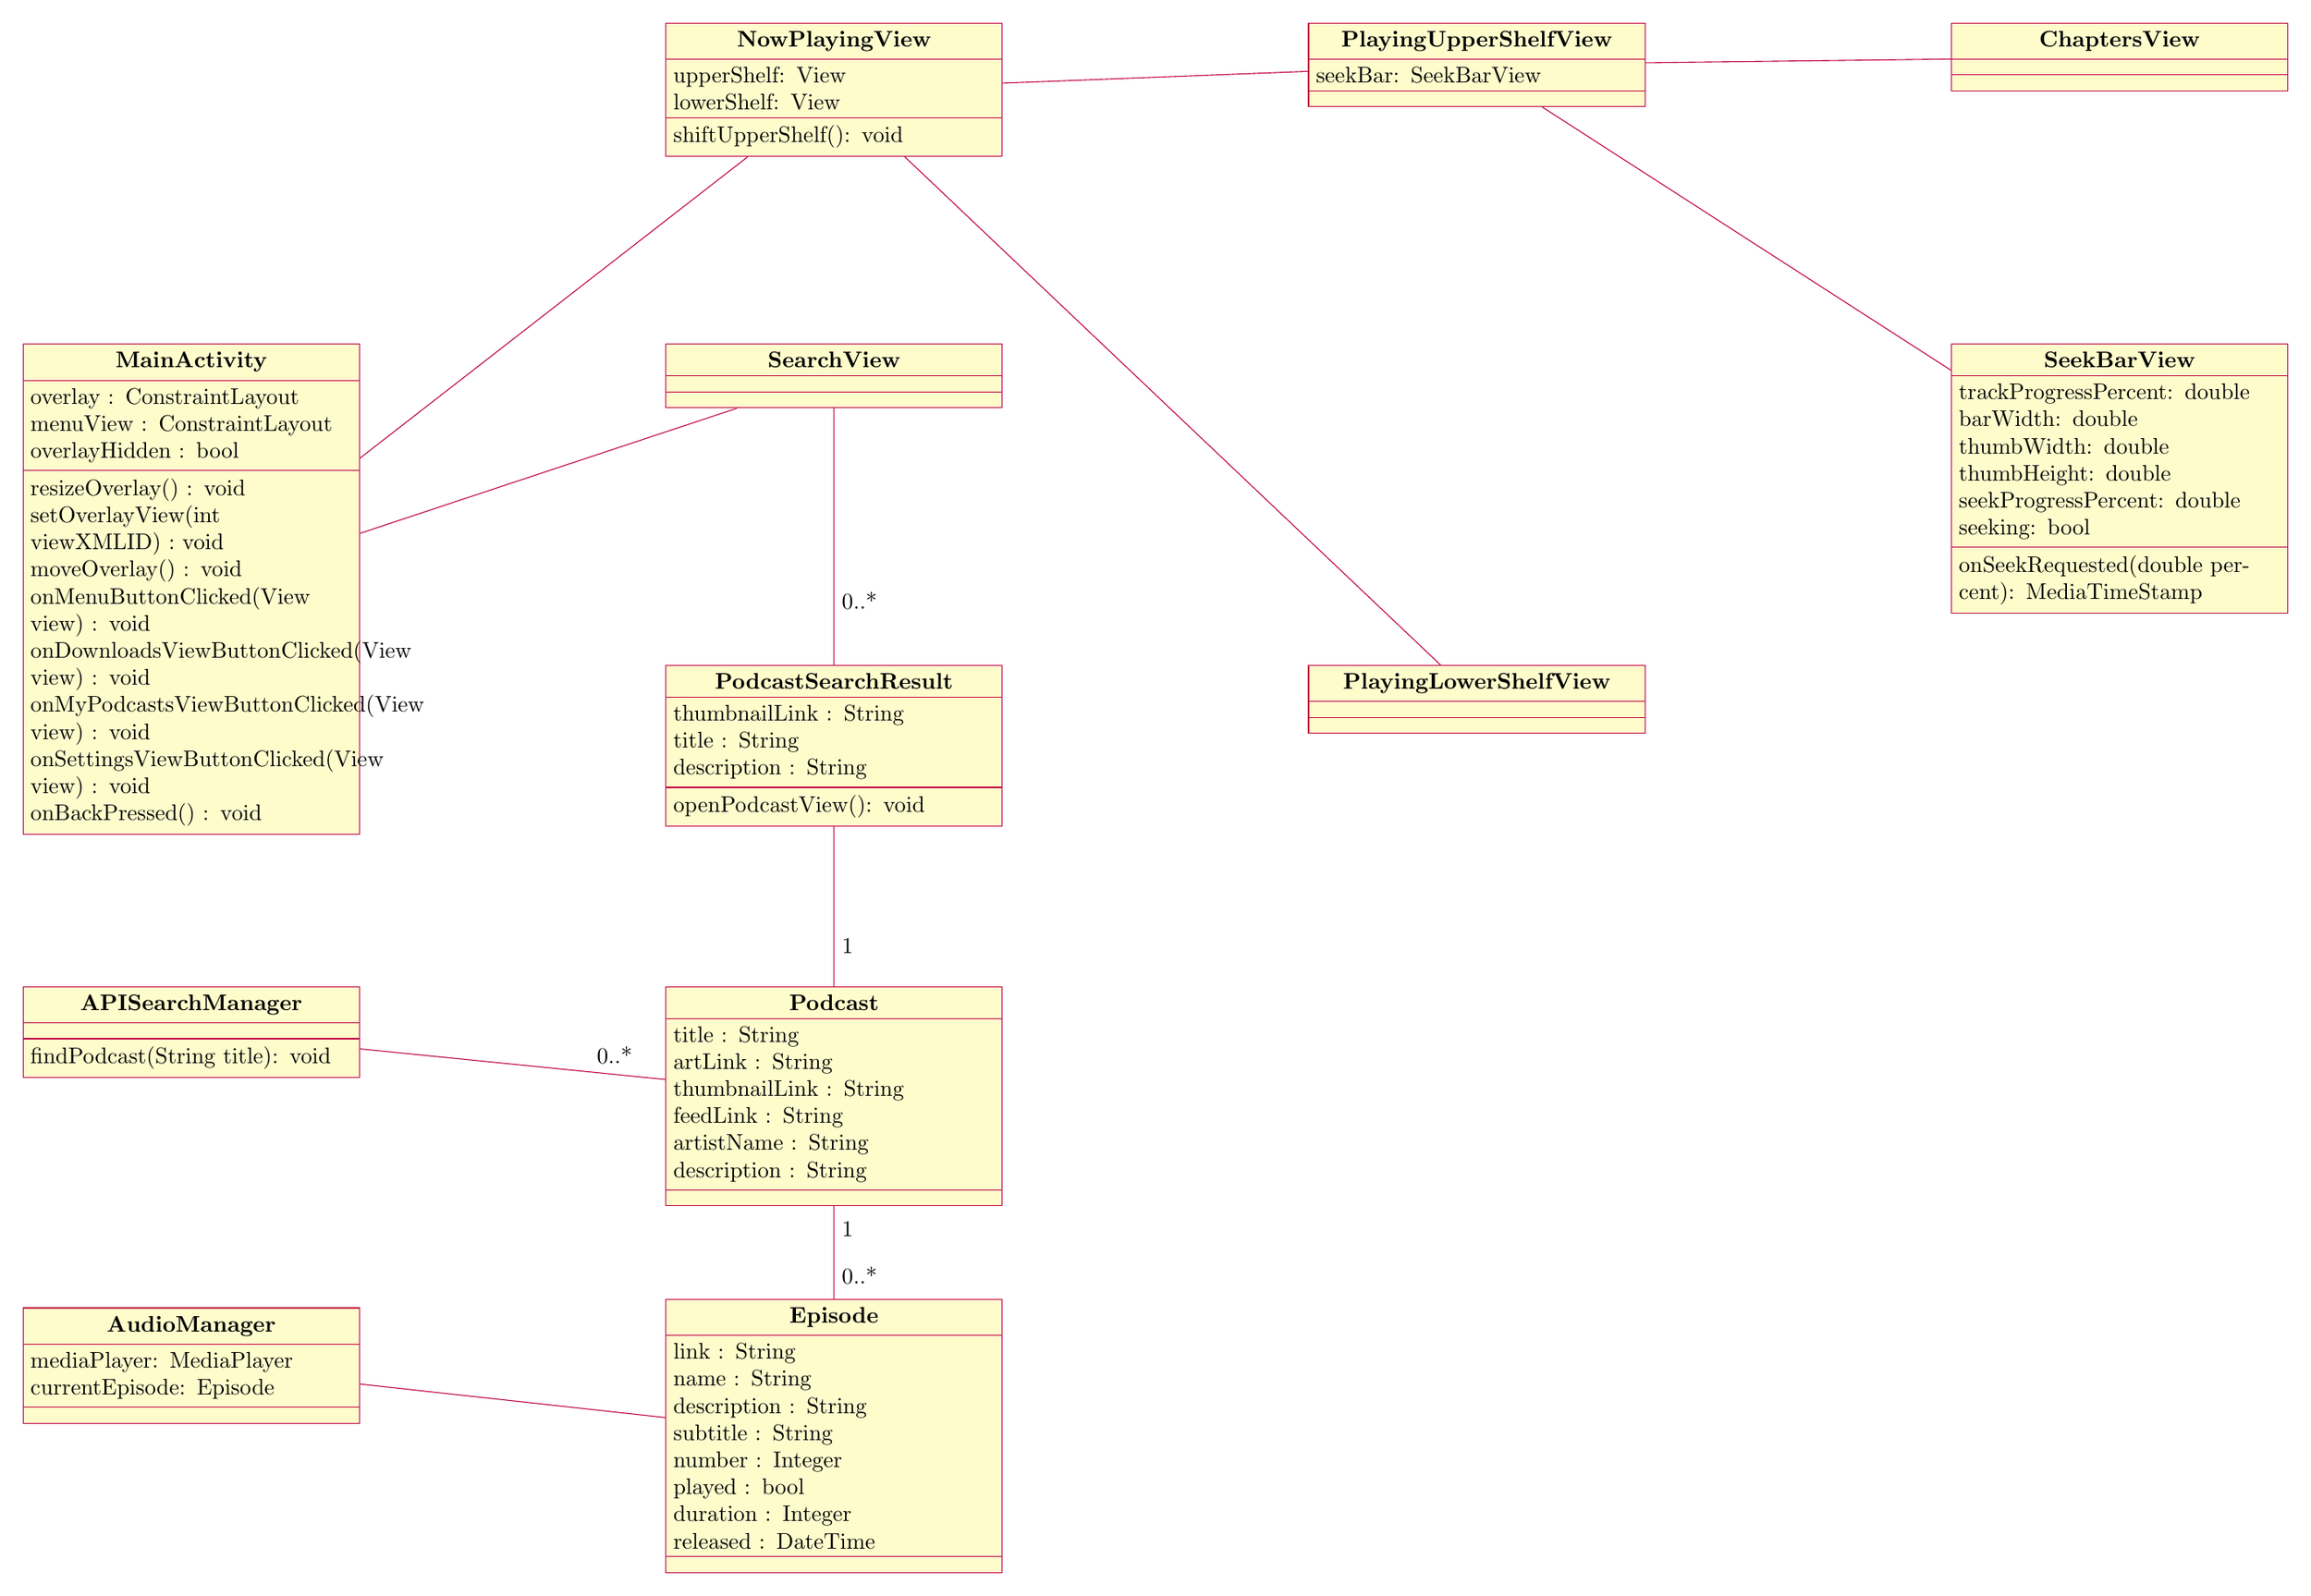
\begin{tikzpicture}[node distance=5cm]
      % MainActivity:
      %   Contains the other views and activities
      \begin{class}{MainActivity}{0, 0}
        \attribute{overlay : ConstraintLayout}
        \attribute{menuView : ConstraintLayout}
        \attribute{overlayHidden : bool}
        \operation{resizeOverlay() : void}
        \operation{setOverlayView(int viewXMLID) : void}
        \operation{moveOverlay() : void}
        \operation{onMenuButtonClicked(View view) : void}
        \operation{onDownloadsViewButtonClicked(View view) : void}
        \operation{onMyPodcastsViewButtonClicked(View view) : void}
        \operation{onSettingsViewButtonClicked(View view) : void}
        \operation{onBackPressed() : void}
      \end{class}
      % NowPlayingView:
      %   Contains the Upper and Lower shelf views
      \begin{class}{NowPlayingView}{10, 5}
        \attribute{upperShelf: View}
        \attribute{lowerShelf: View}
        \operation{shiftUpperShelf(): void}
        % further methods TBD
      \end{class}
        % PlayingUpperShelfView:
        %   Shows the currently playing podcast's title, description
        %   art, and the SeekBar
        \begin{class}{PlayingUpperShelfView}{20, 5}
          \attribute{seekBar: SeekBarView}
        \end{class}
          % ChaptersView:
          %   Displays all of the chapter related tag/metadata information
          %   on the currently playing audio 
          \begin{class}{ChaptersView}{30, 5}
          \end{class}
          % SeekBarView:
          %   Shows the AudioPlayer's progress through the current file
          %   and allows the user to scrub through the file
          \begin{class}{SeekBarView}{30, 0}
            \attribute{trackProgressPercent: double}
            \attribute{barWidth: double}
            \attribute{thumbWidth: double}
            \attribute{thumbHeight: double}
            \attribute{seekProgressPercent: double}
            \attribute{seeking: bool}
            \operation{onSeekRequested(double percent): MediaTimeStamp}
          \end{class}
        % PlayingLowerShelfView:
        %   Contains the player controls, meta operations buttons (fav,
        %   share, show chapters), and ChaptersView
        \begin{class}{PlayingLowerShelfView}{20, -5}
        \end{class}
      % SearchView:
      %   Allows the user to search for a given podcast
      \begin{class}{SearchView}{10, 0}
      \end{class}
      % % DownloadsView:
      % %   Allows the user to view their downloaded podcasts
      % \begin{class}{DownloadsView}{-22, -20}
      % \end{class}
      % % MyPodcastsView:
      % %   Allows the user to view their saved podcasts
      % \begin{class}{MyPodcastsView}{-22, -20}
      % \end{class}
      % % SettingsView:
      % %   Allows the user to view and change general settings
      % \begin{class}{SettingsView}{-22, -20}
      % \end{class}

      % AudioManager:
      %   A singleton which controls the playing of podcast audio
      \begin{class}{AudioManager}{0, -15}
        \attribute{mediaPlayer: MediaPlayer}
        \attribute{currentEpisode: Episode}
        % further methods TBD
      \end{class}
      % APISearchManager:
      %   Handles requests to search for podcast information using the available
      %   web APIs.
      \begin{class}[text width=5cm]{APISearchManager}{0, -10}
        % \attribute{results : ArrayList\textless Podcast\textgreater}
        \operation{findPodcast(String title): void}
      \end{class}
      % PodcastSearchResult:
      %   Represents one result in the list of results displayed when
      %   when searching for a podcast
      \begin{class}[text width=5cm]{PodcastSearchResult}{10, -5}
        \attribute{thumbnailLink : String}
        \attribute{title : String}
        \attribute{description : String}
        \operation{openPodcastView(): void}
      \end{class}
      % Podcast:
      %   describes a whole podcast
      \begin{class}[text width=5cm]{Podcast}{10, -10}
        \attribute{title : String}
        \attribute{artLink : String}
        \attribute{thumbnailLink : String}
        \attribute{feedLink : String}
        \attribute{artistName : String}
        \attribute{description : String}
      \end{class}
      % Episode:
      %   describes a podcast episode
      \begin{class}[text width=5cm, below of=Podcast]{Episode}{10, -15}
        \attribute{link : String}
        \attribute{name : String}
        \attribute{description : String}
        \attribute{subtitle : String}
        \attribute{number : Integer}
        \attribute{played : bool}
        \attribute{duration : Integer}
        \attribute{released : DateTime}
      \end{class}

      \association {MainActivity}{}{}{NowPlayingView}{}{}
      \association {MainActivity}{}{}{SearchView}{}{}
      
      \association {NowPlayingView}{}{}{PlayingUpperShelfView}{}{}
        \association {PlayingUpperShelfView}{}{}{ChaptersView}{}{}
        \association {PlayingUpperShelfView}{}{}{SeekBarView}{}{}
      \association {NowPlayingView}{}{}{PlayingLowerShelfView}{}{}

      \association {SearchView}{}{}{PodcastSearchResult}{0..*}{}

      \association {APISearchManager}{}{}{Podcast}{0..*}{}
      \association {Podcast}{1}{}{Episode}{0..*}{}
      \association {AudioManager}{}{}{Episode}{}{}
      \association {PodcastSearchResult}{}{}{Podcast}{1}{}
    \end{tikzpicture}
\end{document}





